\documentclass{beamer}

\usepackage[ngerman]{babel}

\usepackage[utf8]{inputenc}

\usepackage{hyperref}

\usepackage{tabularx}
\usepackage{array}
\newcolumntype{$}{>{\global\let\currentrowstyle\relax}}
\newcolumntype{^}{>{\currentrowstyle}}
\newcommand{\rowstyle}[1]{\gdef\currentrowstyle{#1}%
	#1\ignorespaces
}
\usepackage{multirow}

\usepackage{listings}
\lstset{
	tabsize=4,
	keywordstyle=\color{blue},
	commentstyle=\color{gray},
	stringstyle=\color{blue},
	alsoletter=0123456789,
}

\newcommand\opstyle{\color{red}} % <--- customise operator style here
\makeatletter
\lstset
{%
  language=C++,
  alsoletter=0123456789,% to prevent \opstyle from being applied to digits
}
% Hook into listings
\lst@AddToHook{OutputOther}{\ProcessOther@silmeth}
% helper macro
\newcommand\ProcessOther@silmeth
{%
  \ifnum\lst@mode=\lst@Pmode%     % If we're in `Processing' mode...
    \def\lst@thestyle{\opstyle}%  % ... redefine the style locally
  \fi%
}
\makeatother


\title{OOP-Vererbung, Polymorphie (Vielgestaltigkeit)}
\author{Paul Raffer}
\date{}

%\setbeamertemplate{footline}{goo \insertframenumber}

\begin{document}

	\maketitle
	
	\section{Polymorphie}
	\begin{frame}
		\frametitle{Polymorphie}
		\begin{table}[h]
	\begin{tabularx}{\textwidth}{$l|^X|^X}
		\rowstyle{\bfseries}  & universell                              & Ad-hoc                             \\
		\rowstyle{\small}     & unendlich viele Typen                   & endliche Anzahl an Typen           \\
		\rowstyle{\small}     & eine Implementierung                    & unterschiedliche Implementierungen \\
		\hline
		\bfseries dynamisch   & \multirow{2}{*}{Inklusionspolymorphie/} & \multirow{3}{*}{Coercion}          \\
		\small    Laufzeit    & \multirow{2}{*}{Vererbungspolymorphie}  &                                    \\
		\small    langsamer   &                                         &                                    \\
		\hline
		\bfseries statisch    & \multirow{2}{*}{parametrische}          & \multirow{3}{*}{Überladung}        \\
		\small    Kompilezeit & \multirow{2}{*}{Polymorphie}            &                                    \\
		\small    schneller   &                                         &                                    \\
	\end{tabularx}
\end{table}

	\end{frame}
	
	
	\begin{frame}
		\frametitle{Geschichte}
		\begin{itemize}
			 \item ...
		\end{itemize}
	\end{frame}
	
	
	\subsection{Vererbungspolymorphie}
	\begin{frame}
		\frametitle{Vererbungspolymorphie}
		\begin{itemize}
			\item Vererbung
			\begin{itemize}
				\item virtuelle Funktionen
				\item abstrakte Klassen
				\item Mehrfachvererbung
				\begin{itemize}
					\item virtuelle Vererbung
				\end{itemize}
			\end{itemize}
		\end{itemize}
	\end{frame}
	
	{\setbeamertemplate{footline}{\vspace*{-8pt}Vollständiges Beispiel: \url{https://godbolt.org/z/heEWxW}}
	\begin{frame}[fragile]
		\frametitle{Beispiel: Formen}
		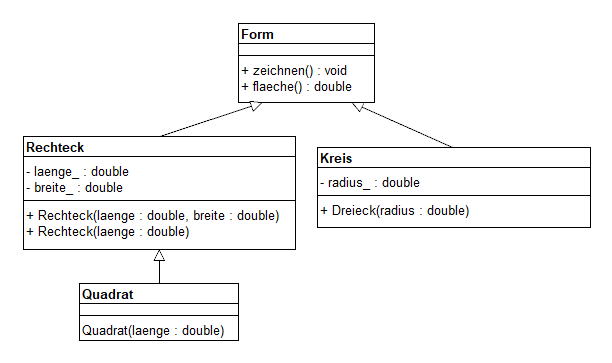
\includegraphics[width=\textwidth]{./res/polymorphie/universell/vererbung/form/uml.png}
	\end{frame}
	
	{\setbeamertemplate{footline}{\vspace*{-8pt}Vollständiges Beispiel: \url{https://godbolt.org/z/heEWxW}}
	\begin{frame}[fragile]
		\frametitle{Beispiel: Formen}
		\UseRawInputEncoding
		\pause{\tiny\lstinputlisting[language={C++}]{./res/polymorphie/universell/vererbung/form/src/form.hpp}}
		\pause{\tiny\lstinputlisting[language={C++}]{./res/polymorphie/universell/vererbung/form/src/rechteck.hpp}}
		\pause{\tiny\lstinputlisting[language={C++}]{./res/polymorphie/universell/vererbung/form/src/quadrat.hpp}}
		\pause{\tiny\lstinputlisting[language={C++}]{./res/polymorphie/universell/vererbung/form/src/kreis.hpp}}
		\inputencoding{utf8}
		
	\end{frame}
	}
	
	\begin{frame}
		\frametitle{Mehrfachvererbung}
		\begin{itemize}
			\item Funktionalität von mehreren Klassen kombinieren
		\end{itemize}
	\end{frame}
	
	{\setbeamertemplate{footline}{\vspace*{-8pt}Vollständiges Beispiel: \url{https://godbolt.org/z/heEWxW}}
	\begin{frame}[fragile]
		\frametitle{Virtuelle Vererbung}
		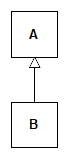
\includegraphics[height=0.8\textheight]{./res/polymorphie/universell/vererbung/virtuell/uml.png}
	\end{frame}
	
	
	\subsection{Coercion}
	\subsubsection{eingebaute Datentypen}
	{\setbeamertemplate{footline}{\vspace*{-8pt}Vollständiges Beispiel: \url{https://godbolt.org/z/}}
	\begin{frame}
		\frametitle{Coercion}
		\begin{itemize}
			\item implizite Typumwandlungen
			\begin{itemize}
				\UseRawInputEncoding
				
				\pause\item eingebaute Datentypen
					{\tiny\lstinputlisting[language={C++}]{./res/polymorphie/adhoc/coercion/src/eingebauteDatentypen.cpp}}
				\pause\item eingene Datentypen
				\begin{itemize}
					\pause\item Konvertierungskonstruktoren
						{\tiny\lstinputlisting[language={C++}]{./res/polymorphie/adhoc/coercion/src/konvertierungskonstruktoren.cpp}}
					\pause\item Konvertierungsoperatoren
						{\tiny\lstinputlisting[language={C++}]{./res/polymorphie/adhoc/coercion/src/konvertierungsoperatoren.cpp}}
				\end{itemize}
				\inputencoding{utf8}
			\end{itemize}
		\end{itemize}
	\end{frame}
	}
	
	
	\subsection{parametrische Polymorphie}
	\begin{frame}
		\frametitle{parametrische Polymorphie}
		\begin{itemize}
			\item Templates/Generics
			\begin{itemize}
				\item Funktionstemplates
				\item Klassentemplates
				\item Konzepte
			\end{itemize}
		\end{itemize}
	\end{frame}
	
	{\setbeamertemplate{footline}{\vspace*{-8pt}Vollständiges Beispiel: \url{https://godbolt.org/z/}}
	\begin{frame}
		\frametitle{Funktionstemplates}
		\UseRawInputEncoding
		{\tiny\lstinputlisting[language={C++}]{./res/polymorphie/universell/parametrisch/src/funktionstemplates.cpp}}
		\inputencoding{utf8}
	\end{frame}
	}
	
	{\setbeamertemplate{footline}{\vspace*{-8pt}Vollständiges Beispiel: \url{https://godbolt.org/z/}}
	\begin{frame}
		\frametitle{Klassentemplates}
		\UseRawInputEncoding
		\pause{\tiny\lstinputlisting[language={C++}]{./res/polymorphie/universell/parametrisch/src/klassentemplates/stack/1.hpp}}
		\pause{\tiny\lstinputlisting[language={C++}]{./res/polymorphie/universell/parametrisch/src/klassentemplates/stack/2.hpp}}
		\pause{\tiny\lstinputlisting[language={C++}]{./res/polymorphie/universell/parametrisch/src/klassentemplates/stack/3.hpp}}
		\pause{\tiny\lstinputlisting[language={C++}]{./res/polymorphie/universell/parametrisch/src/klassentemplates/stack/4.hpp}}
		\inputencoding{utf8}
	\end{frame}
	}
	{\setbeamertemplate{footline}{\vspace*{-8pt}Vollständiges Beispiel: \url{https://godbolt.org/z/}}
	\begin{frame}
		\frametitle{Klassentemplates}
		\UseRawInputEncoding
		{\tiny\lstinputlisting[language={C++}]{./res/polymorphie/universell/parametrisch/src/klassentemplates/main/1.cpp}}
		\pause{\tiny\lstinputlisting[language={C++}]{./res/polymorphie/universell/parametrisch/src/klassentemplates/main/2.cpp}}
		\pause{\tiny\lstinputlisting[language={C++}]{./res/polymorphie/universell/parametrisch/src/klassentemplates/main/3.cpp}}
		\inputencoding{utf8}
	\end{frame}
	}
	
	
	
	\subsection{Überladung}
	\begin{frame}
		\frametitle{Überladung}
		\begin{itemize}
			\item Funktionsüberladungen
			\begin{itemize}
				\item Operatorüberladungen
			\end{itemize}
		\end{itemize}
	\end{frame}
	
	
	{\tiny
	\begin{frame}
		\frametitle{Quellen}
		\begin{itemize}
	\item FSST-Mitschrift der 2. und 3. Klasse
	\item \url{https://www.ics.uci.edu/~jajones/INF102-S18/readings/05_stratchey_1967.pdf}
	\item \url{https://www.youtube.com/watch?v=uTxRF5ag27A&list=PLrAXtmErZgOdP_8GztsuKi9nrraNbKKp4}
	\item \url{https://soundcloud.com/lambda-cast}
	\item \url{https://de.wikipedia.org/wiki/Polymorphie_(Programmierung)}
	\item \url{https://lec.inf.ethz.ch/ifmp/2019/slides/lecture14.handout.pdf}
	\item \url{https://courses.cs.washington.edu/courses/cse331/11wi/lectures/lect06-subtyping.pdf}
	\item \url{https://de.wikipedia.org/wiki/Vererbung_(Programmierung)}
	\item \url{https://wiki.haskell.org/Polymorphism}
	\item \url{http://lucacardelli.name/Papers/OnUnderstanding.A4.pdf}
	\item C++ Templates: The Complete Guide
	\item C++: Das umfassende Handbuch
	\item Grundkurs C++
	\item C++: Die Sprache der Objekte
	\item Exceptional C++: 47 engineering puzzles, programming problems, and solutions
	\item Effektiv C++. 50 Specific Ways to Improve Your Programs and Designs
	\item \url{https://www.youtube.com/watch?v=HddFGPTAmtU}
	\item \url{https://www.bfilipek.com/2020/04/variant-virtual-polymorphism.html}
	\item \url{https://de.wikipedia.org/wiki/Diamond-Problem}
\end{itemize}

	\end{frame}
	}
	
\end{document}
